\documentclass[norsk]{uiobachelorthesis}
\usepackage[utf8]{inputenc}
\usepackage[T1]{fontenc, url}   \urlstyle{sf}
\usepackage{babel, textcomp}
\usepackage{amsmath}
\usepackage{graphicx}
\usepackage{csquotes}
\usepackage{tikz}
\usepackage{enumitem}
\usepackage{placeins}
\usetikzlibrary{positioning, arrows.meta, fit}
\usepackage[backend=biber, style=authoryear]{biblatex}
\addbibresource{kilder.bib}

\title{A rust application for displaying live network quality graphs\\[1ex]
  \large A tool for displaying live data from a WI-FI network to give the user an overview of the current network conditions}
\author{Vegard Myklebust\\ \url{vamykleb@ifi.uio.no}}
\date{IN3260 \\ \today}

\begin{document}
\maketitle

\begin{abstract}
\end{abstract}

\tableofcontents
\newpage

\section{Introduksjon}
\label{sec:introduksjon}
Denne oppgaven bygger på prosjektet til veilederen min, som måler ulike latens-tider i et datanettverk. Resultatet er en linje med målinger per ramme. Da det kan komme mange målinger i sekundet er det vanskelig å få et bilde av hvordan nettverket oppfører seg til enhver tid gjennom en visning i terminalen. Det trengs derfor ett verktøy som kan vise frem disse målingen grafisk mens de kommer inn. prosjektet er også skrevet  i programmeringsspråket Rust som er det samme som veilederen min har brukt til måleprogrammet. 
 %TODO skriv bedre vegard
% Problem, motivasjon og mål: hvorfor live CDF av latens per MAC-par? Avslutt med hva rapporten viser.
%kontektst, porble
%hva jeg har laget
%mål
%rammer og avgrensinger?
%oversikt over rapporten
%Hver retning måles separat
% skrive bedre om forsikelser på nettet

\subsection{Bakgrunn}
\label{sec:bakgrunn}
	\subsubsection{Latens}
	\label{sec:latens}
I dette prosjektet måler måleverktøyet tiden en ramme bruker på tre forskjellige faser gjennom et Wi-Fi-nettverk. Latens blir målt i mikrosekunder (\textmu{}s) og vises i millisekunder (ms). Her blir sender og mottaker identifisert med MAC-adresser. Det gjør også at hver retning måles for seg, siden forsinkelsen kan være ulik i de to retningene. I et Wi-Fi-nettverk varierer latensen mer enn i fysiske nettverkskabler siden signaler ofte møter på fysiske hindringer, som kan føre til rammetap eller gjensendinger av rammer. Grunnen til at måleverktøyet måler forsinkelsen i tre forskjellige faser er for å finne ut hvor forsinkelsen oppstår. De tre fasene er: 
\begin{itemize}
\item [-] før sending (RTS/CTS-prelude)
\item [-] under sending (Gjensending)
\item[-] etter mottak (Reordering)
\end{itemize}
RTS/CTS-prelude måler latensen fra før en ramme blir sendt. CSMA/CA er en protokoll som brukes i Wi-Fi for å forebygge kollisjoner. I CSMA/CA brukes RTS/CTS for å reservere tilgang til kanalen. Dette må skje slik at to sendere ikke ødelegger for hverandres sendinger, ved at rammene kolliderer med hverandre. Dette oppstår ved at de to senderne ikke hører hverandre sende. Dette kalles skjult node-problemet. RTS er en \enquote{forespørsel om å sende} (Request to Send). CTS står for \enquote{klar til å sende} (Clear to Send). Det vil si at mottaker sender en melding om at mottakeren er opptatt og at alle rundt må være stille. Dette løser skjult node-problemet med at CTS når alle i nærheten av mottakeren, også de som ikke hørte RTS-en \parencite[avsnitt~7.3.1]{kurose2025}. Forsinkelser her oppstår ved høy trafikk på nettverket når mange prøver å sende RTS. Dette vil da føre til at det blir kollisjoner med avsendere som også vil sende. De venter da en kort fast tid på å motta en CTS. Når den ikke kommer, sender de en ny RTS etter et tilfeldig valgt tidsintervall (backoff). Måleverktøyet måler tiden det tar fra RTS er sendt til avsenderen får tilbake en CTS. Dette blir målt med feltet \texttt{rts\_cts\_prelude\_pcap\_delta}. 
%riktig med at det er fra RTS er sendt til CTS blir mottat?

ACK brukes for å vise at rammen kommer fram til mottakeren. Etter å ha sendt rammen venter avsenderen på at mottakeren sender tilbake en ACK. At ACK uteblir, kan skyldes fysiske hindringer, stor avstand mellom avsenderen og mottakeren, forstyrrelser eller kollisjoner med andre sendere. Avsenderen venter en fast tid på å motta en ACK. Hvis ACK-en ikke kommer, venter avsenderen en tilfeldig backoff før rammen sendes på nytt. Backoff-intervallet øker for hver gjensending som gjennomføres. Etter et visst antall sendeforsøk gir avsenderen opp \parencite{kurose2025}. Når en ramme må bli sendt på nytt, sendes den med samme sekvensnummer og retry-biten settes til 1. Måleverktøyet bruker disse to til å kjenne igjen forsøk som samme ramme. Feltet \texttt{latency\_pcap\_delta} er tiden fra første til siste forsøk. 

Fra Wi-Fi-standarden 802.11n og utover blir rammene aggregert sammen og kvittert med en Block ACK, i stedet for at en og en ramme blir ACK-et. Aggregering brukes siden det tar mye tid å få tilgang til en kanal, derfor er det best å sende mange rammer samtidig. Block ACK sender kvittering for alle rammene som kom fram. Ut fra dette vil avsender vite hvilke  som ikke kom fram og sende dem på nytt \parencite[s.~38]{gast2013}. Siden rammene må bli levert videre opp til IP-laget i riktig rekkefølge, holder mottakeren rammene i en reorder-buffer og bruker sekvensnummer til å sortere dem \parencite{ieee80211-2020}. Rammene som kommer etter den manglende rammen blir ventende fram til den manglende rammen kommer og settes på riktig plass. De må vente, selv om de kom fram på første forsøk. Måleverktøyet måler tiden rammene venter på reordering med \texttt{reordering\_delay\_pcap\_delta}. Denne viser tiden fra rammen kom fram, til alle tidligere rammer har kommet fram.
%se på kilder her



	\subsubsection{Kumulativ fordelingsfunksjon (CDF)}
	\label{sec:cdf}
		En kumulativ fordelingsfunksjon (CDF) gir sannsynligheten for at en tilfeldig variabel er mindre enn eller lik en 				spesifisert verdi \parencite{wasserman2006}.
		\begin{equation} 
			F(x) = P(X \le x) 
			\label{eq:cdf}
		\end{equation}
		$X$ er latensen til en tilfeldig måling for et gitt MAC-par (tilfeldig variabel). $x$ er en vilkårlig latensverdi på x-aksen og grafen viser $F(x)$ for alle verdier av $x$. I CDFen går $F$ fra 0 til 1 der 1 er 100\,\% og 0 er 0\,\%. Siden det bare finnes et utvalg med målinger, er den sanne fordelingen $F$ ukjent. Derfor må $F$ estimeres med dataene
med en empirisk CDF (ECDF). ECDF teller hvor mange målinger som er $\le x$ og deler på $n$, altså andelen som er $\le x$.

\begin{equation}
  \hat{F}_n(x) = \frac{1}{n} \sum_{i=1}^{n} \mathbf{1}\{x_i \le x\}
  \label{eq:ecdf}
\end{equation}
\begin{itemize}

\item[-] $n$: antall målinger.
\item[-] $x_i$: de målte latensene.
\item[-] $x$: verdiene funksjonen evalueres i, altså et punkt på x-aksen.
\item[-] $\hat{F}_n(x)$: estimatet. \enquote{Hatten} betyr at det er et estimat og $n$ at det bygger på $n$ målinger.
\item[-]$\mathbf{1}\{x_i \le x\}$: \enquote{funksjonen}, som er 1 hvis betingelsen er sann og 0 ellers.
\end{itemize}

Egenskapene til en ECDF er en trappefunksjon som hopper med $1/n$ ved hver måling (n).
Den går fra 0, når $x$ er lavere enn den minste målingen, til 1, når $x$ er større enn eller lik den største.
ECDF vil nærme seg den sanne $F$ når $n$ vokser (Glivenko-Cantelli) \parencite{wasserman2006}. 

%skrive noe om ecdf i praksis?
Det som gjør at CDF blir brukt til å vise frem latens, er at man får en bra oversikt over all forsinkelsen i en og samme graf, hvor y-aksen viser prosent av målinger som har mindre enn den latensen (x-aksen).%forklar mer her
	

\subsection{Krav}
\label{sec:krav}
% Kravene fra veileder: CSV-strøm på stdin, generator med tilfeldige forsinkelser,
% pipe ./generator | ./gui, egen tråd som leser stdin, anbefalte crates.
Dette prosjektet har blitt veiledet av Magnus Skjegstad som har gitt meg oppgaver gjennom semesteret. Oppgaven startet med å skulle utvikle en GUI til et allerede eksisterende verktøy for måling av latensverdier i et nettverk. Denne videreutviklingen skulle gjøre dataene fra måleprogrammet lettere å avlese som en GUI istedenfor rett fra terminalen.  
\begin{enumerate}[label=K\arabic*]
  \item \label{krav:stdin} Programmet skal lese data som en strøm fra stdin, som en måling per linje i CSV-format
  %er det csv-format 
  \item \label{krav:pipe} Programmet skal kobles sammen med en pipe \texttt{(./generator | ./gui)}
  \item \label{krav:trad} GUI-en skal ha en egen tråd som leser stdin 
  \item \label{krav:testprogram} Det skal finnes et testprogram som genererer testdata
  \item \label{krav:cdf} Programmet skal vise live CDF per MAC-par, med hver retning for seg
  \item \label{krav:sek} CDF skal kun vise de siste 60 sekundene med målinger
  \item \label{krav:statistikk} Programmet skal ha en oversikt over parene med statistikk (median, snitt, p95, p99, maks)
  \item \label{krav:klikkforvise} Skal være mulig å bare vise ett par ved klikk på det
  \item \label{krav:rust} Koden skal være skrevet i Rust
\end{enumerate}

Underveis i utviklingen av programmet anbefalte veilederen bruken av chrono, tokio, csv og serde. Dette var mer råd enn krav.
% dårlig settning ja

\section{Metode}
\label{sec:metode}
% Nok detaljer til at andre kan gjenskape løsningen.

\subsection{Arkitektur}
\label{sec:arkitektur}
% Innledende avsnitt + figur
Prosjektet er skrevet i Rust og er delt inn i to deler. Den ene delen er \texttt{live\_cdf}, som tar inn et dataformat som inndata og gjør det til en CDF-graf og statistikk. Den andre delen av programmet er en \texttt{csv\_streamer} som leser data fra en testfil som er på samme format som de ekte dataene. Disse to programmene er koblet sammen med en UNIX-pipe, som oppfyller krav~\ref{krav:pipe}. Programmet ligger i et Cargo-workspace noe som gjør at man kan dele et større prosjekt i flere mindre pakker (crates). \texttt{live\_cdf}-programmet bruker to tråder: en for å kunne lese og beregne dataen, og en som viser dataen, som oppfyller krav~\ref{krav:trad}. Dataflyten i programmet vil se ut som Figur~\ref{fig:arkitektur} ved bruk av CSV-fil for å teste programmet. Siden \texttt{live\_cdf} ikke bryr seg om hvor dataen kommer fra, bare hvordan den ser ut, kan man hoppe over \texttt{csv\_streamer} og sende data direkte til \texttt{live\_cdf}. Det er en delt type i programmene som er \texttt{TRow} i pakken \texttt{felles} som er formatet på inndataen. Det er dette som gjør at begge programmene er enige om hvilket format dataene har.

\begin{figure}[htbp]
\centering
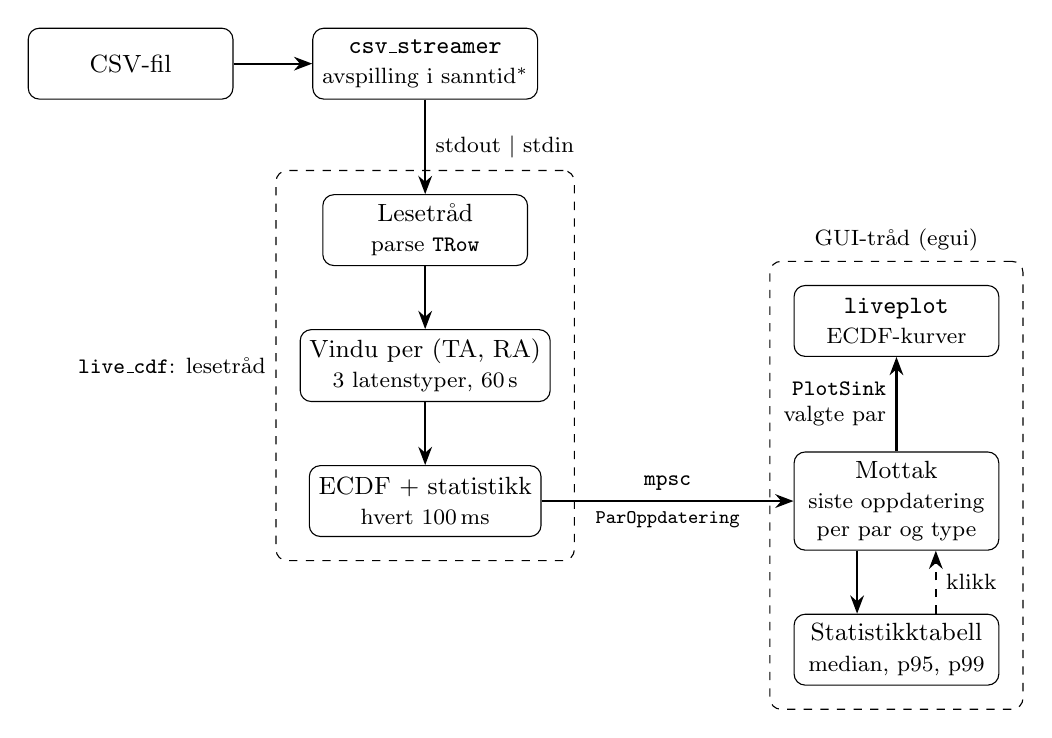
\begin{tikzpicture}[
  node distance=8mm and 10mm,
  boks/.style={draw, rounded corners, align=center, minimum height=9mm,
               minimum width=26mm, font=\small},
  pil/.style={-{Stealth}, thick},
  ramme/.style={draw, dashed, inner sep=3mm, rounded corners}
]
% Noder i lesetråden (venstre kolonne)
\node[boks] (fil) {CSV-fil};
\node[boks, right=of fil] (streamer) {\texttt{csv\_streamer}\\\footnotesize avspilling i sanntid$^{*}$};
\node[boks, below=12mm of streamer] (leser) {Lesetråd\\\footnotesize parse \texttt{TRow}};
\node[boks, below=of leser] (lagring) {Vindu per (TA, RA)\\\footnotesize 3 latenstyper, 60\,s};
\node[boks, below=of lagring] (beregn) {ECDF + statistikk\\\footnotesize hvert 100\,ms};

% Noder i GUI-tråden (høyre kolonne)
\node[boks, right=32mm of beregn] (mottak) {Mottak\\\footnotesize siste oppdatering\\[-1pt]\footnotesize per par og type};
\node[boks, above=12mm of mottak] (plot) {\texttt{liveplot}\\\footnotesize ECDF-kurver};
\node[boks, below=of mottak] (tabell) {Statistikktabell\\\footnotesize median, p95, p99};

% Stiplete rammer rundt trådene
\node[ramme, fit=(leser)(lagring)(beregn),
      label={[font=\footnotesize]left:\texttt{live\_cdf}: lesetråd}] {};
\node[ramme, fit=(plot)(mottak)(tabell),
      label={[font=\footnotesize]above:GUI-tråd (egui)}] {};

% Piler (dataflyt)
\draw[pil] (fil) -- (streamer);
\draw[pil] (streamer) -- node[right, font=\footnotesize]{stdout $\mid$ stdin} (leser);
\draw[pil] (leser) -- (lagring);
\draw[pil] (lagring) -- (beregn);
% Kanal mellom trådene: én melding per serie med ECDF-punkter og statistikk
\draw[pil] (beregn) -- node[above, font=\footnotesize]{\texttt{mpsc}}
                       node[below, font=\scriptsize]{\texttt{ParOppdatering}} (mottak);
% Inne i GUI-tråden
\draw[pil] (mottak) -- node[left, font=\footnotesize, align=right]{\texttt{PlotSink}\\valgte par} (plot);
\draw[pil] ([xshift=-5mm]mottak.south) -- ([xshift=-5mm]tabell.north);
% Brukervalg: klikk i tabellen bestemmer hvilke par som tegnes
\draw[pil, dashed] ([xshift=5mm]tabell.north) -- node[right, font=\footnotesize]{klikk} ([xshift=5mm]mottak.south);
\end{tikzpicture}
\caption{
Dataflyt i programmet. Data spilles av fra fil av \texttt{csv\_streamer}, sendes gjennom en pipe til \texttt{live\_cdf}, der en lesetråd beregner ECDF og statistikk og sender resultatet til GUI-tråden. \\
{\footnotesize $^{*}$Radene sendes med samme tidsavstand som mellom pakkene i CSV-filen (differansen i \texttt{first\_seen\_pcap\_ts}).}}
\label{fig:arkitektur}
\end{figure}


  \subsubsection{Avspilling av data}
  \label{sec:avspilling}
  \texttt{csv\_streamer} leser målinger fra CSV-fil med målinger som er laget med samme header som de \enquote{ekte} målingene vil ha. Headeren har feltene som ligger i \texttt{TRow}. Feltet \texttt{first\_seen\_pcap\_ts} er tidspunktet rammen først ble sett, i \textmu{}s. De tre latensverdiene er forklart i bakgrunnskapitlet (avsnitt~\ref{sec:latens}). Det blir brukt testfiler i form av csv siden det ikke var mulig å få tak i reelle data underveis i utviklingen. En annen grunn til å bruke testdata er at det blir lettere å se om alt stemmer underveis. Først ble programmet testet med en generator som skrev tilfeldige latensverdier til stdout, slik krav~\ref{krav:testprogram} beskriver. Da simuleringsfilene med samme format som måleverktøyet kom, ble generatoren byttet ut med \texttt{csv\_streamer}, som spiller av disse filene. Simuleringsfilene har alle tre latenstypene og mer realistiske verdier enn tilfeldige tall, og de sendes fortsatt til \texttt{live\_cdf} gjennom en pipe (krav~\ref{krav:pipe}). Radene sendes med samme tidsavstand som i filen. Ellers ville all dataen kommet med en gang og programmet ville da ikke oppført seg som med \enquote{ekte} data. Ettersom CSV-filen simulerer \enquote{live} data, vil visningsvinduet på 60 s og oppdateringsfrekvensen på 100 ms gi korrekt visning. Hele \texttt{csv\_streamer} skriver til stdout og kan derfor bli byttet ut med den ekte kilden til dataen uten endringer i \texttt{live\_cdf}.
  
    
\subsubsection{Innlesing og beregning}
\label{sec:innlesning}
Grunnen til at innlesing og beregningene av CDF og statistikk skjer på en egen tråd og ikke på samme som GUI, er at stdin blokkerer mens den venter på data. GUI-en skal tegne 60 ganger i sekundet. Dette vil gjøre at GUI-en fryser, hvis den også må vente på inndata og at beregninger skal bli ferdig (krav~\ref{krav:trad}). Her har jeg valgt å bruke \texttt{std::thread} istedenfor \texttt{tokio}. Når programmet kun lager én tråd for innlesing av data (stdin) så fører tokio kun til at det blir mer overhead fordi tokio er bedre når man skal ha mange samtidige oppgaver (tasks) \parencite{tokio_tutorial}. Tokio leser også stdin med en vanlig blokkerende tråd derfor hadde man ikke fått noe gevinst av å bruke tokio her \parencite{tokio_stdin}.

Programmet tolker en innkommende rad som \texttt{TRow}. Radene blir gruppert etter par \texttt{(TA,RA)} hvor retningen teller (krav~\ref{krav:cdf}). Hvert par har tre serier, én per latenstype som i avsnitt~\ref{sec:latens}.

CDF-en har et glidende vindu det vil si at den kun viser målingene for de siste 60 sekundene i datatid (tid basert på tidsstemplene i dataene, ikke sanntid), målt etter \texttt{first\_seen\_pcap\_ts}. Hvis en måling er eldre enn 60 sekunder vil den bli fjernet fra utregningene. Dette er for å vise hvordan nettverket oppfører seg nå (krav~\ref{krav:sek}). Dette gjør også at programmet oppfører seg likt både ved avspilling av testdata og med live data.

Når ECDF og statistikk skal beregnes, velger jeg å kun gjøre det hvert 100 ms sanntid, og kun når en serie har endret seg. Her bruker jeg sanntid siden oppdateringen er for den som ser på, og derfor må den følge vanlig tid. Dette gjøres fordi hvis programmet skulle beregnet dataen for hver rad som kommer inn, ville dette ført til mange tusener ekstra beregninger som det ikke er mulig å se. 100 ms vil fortsatt se \enquote{live} ut.
%endre til 1000ms for hver oppdateering i programmet?
Når dette er gjort sender lesetråden en melding per serie med ECDF-punkter og statistikk med median, snitt, p95, p99 og maks sendt som en melding over en kanal (\texttt{mpsc}) til GUI-tråden. Jeg bruker meldinger til å sende data i stedet for \texttt{Mutex} siden GUI-tråden aldri skal måtte vente på en lås for å lese dataene \parencite{rustbook-mpsc}.
 
\subsubsection{Brukergrensesnitt}
GUI-en er laget med eframe/egui, som er \emph{immediate mode}: hele vinduet tegnes på nytt hver frame, cirka 60 ganger i sekundet. Hver frame henter GUI-en alle nye meldinger uten å vente (\texttt{try\_recv}). Hvis det ikke kommer noen meldinger, tegner den det den har fra før. Dette og avsnitt~\ref{sec:innlesning} gjør at GUI-en aldri fryser, selv når det ikke kommer noen data inn.

Mottak-delen i figur~\ref{fig:arkitektur} tar vare på den sist mottatte meldingen for hvert par og hver latenstype. Eldre meldinger erstattes. Dette skjer for at GUI-en skal vise tilstanden til nettverket, ikke historikk. Siden historikken ligger i lesetråden trenger ikke GUI-en å holde på annet enn den siste meldingen.

Oppsettet til GUI-en er at statistikktabellen står til venstre og ECDF-grafen tar resten (figur~\ref{fig:gui}). Tabellen har kolonnene Fra, Til, Type, Median, Avg, P95, P99 og Max, og oppfyller krav~\ref{krav:statistikk}. Hver rad har en fargeprikk lik den tilhørende kurven, siden grafen ikke har noen forklaring selv. Grafen viser en kurve per par og latenstype, med latens på x-aksen og andelen som går fra 0 til 1 på y-aksen (se avsnitt~\ref{sec:cdf}). Dette oppfyller krav~\ref{krav:cdf}. Her har jeg brukt \texttt{liveplot} til visning av grafen, siden den hadde mange ferdige funksjoner som zoom, flytting og tilpassing av aksene, og tar imot data over en kanal. Dette kom etter anbefaling fra veileder. 

Et klikk på et par i statistikktabellen slår av eller på visning av grafene (krav~\ref{krav:klikkforvise}). Om ingen par er valgt så vises alle. Når man trykker på et par vises alle tre latenstypene for paret. Dette er fordi grafen blir uleselig når mange par vises samtidig.

\begin{figure}[htbp]
	\centering
	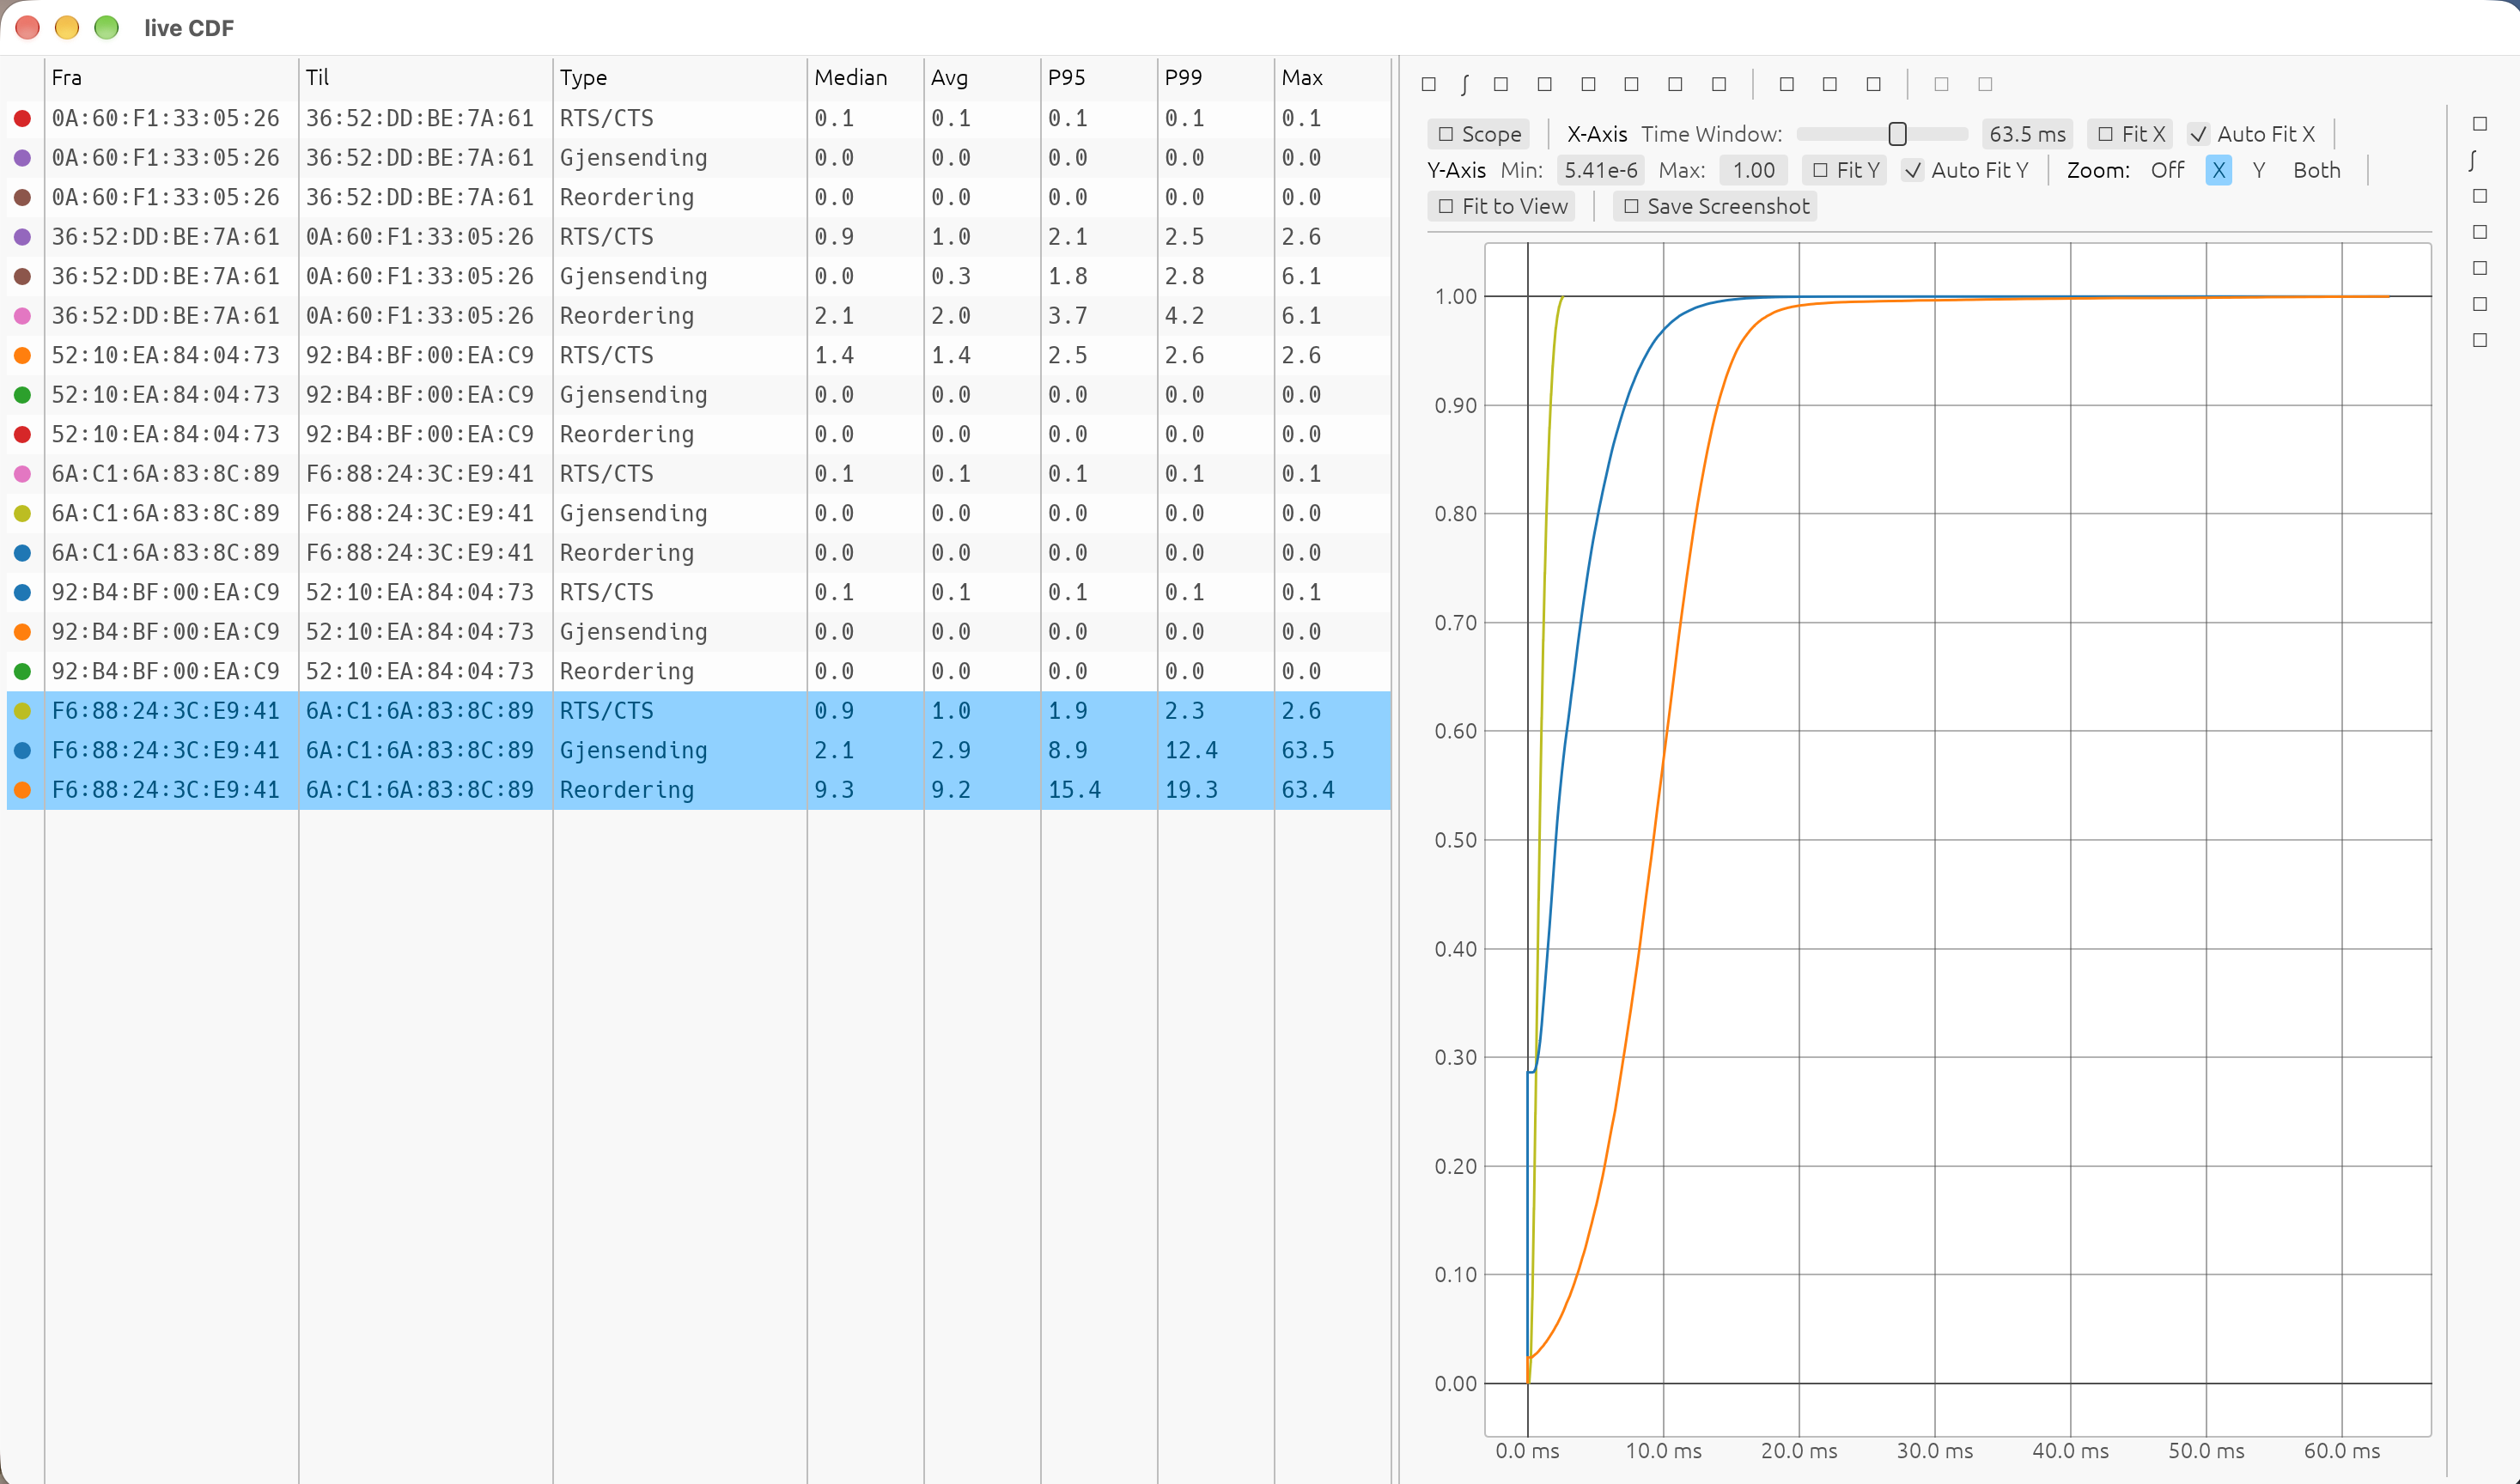
\includegraphics[width=\textwidth]{pictures/CDF-med-en-valgt.png}
	\caption{Skjermbilde av programmet med data fra de tre testfilene. Til venstre statistikktabellen (verdier i ms), til høyre ECDF-kurvene for det valgte paret \texttt{F6:88:24:3C:E9:41} $\rightarrow$ \texttt{6A:C1:6A:83:8C:89} (markert i tabellen). Fargeprikkene foran hver rad viser hvilken kurve raden hører til.}
	\label{fig:gui}
\end{figure}

\FloatBarrier
\subsection{Implementasjon}
\label{sec:implementasjon}
% Datastruktur per MAC-par, beregning av ECDF (sortering, i/n), set_data-intervall,
% 60-sekunders glidende vindu og fjerning av gamle målinger. Verktøy og crates.

Arkitektur (avsnitt~\ref{sec:arkitektur}) har forklart hva og hvorfor, og implementasjon skal beskrive hvordan løsningen er laget, slik at andre kan gjenskape den. Underseksjonene følger samme rekkefølge som arkitektur og dataflyten i figur~\ref{fig:arkitektur}. 

\subsubsection{Workspace og pakker}
\label{sec:impl-workspace} 
% felles, csv_streamer, live_cdf og hvilke crates hver bruker
Prosjektet er et Cargo-workspace med tre pakker (beskrevet i avsnitt~\ref{sec:arkitektur}), hvor alle bruker \texttt{edition = "2024"}. 
Tabell~\ref{tab:pakker} viser pakkene og hvilke crates de bruker. 
\begin{table}[htbp]
\centering
\caption{Pakkene i workspace-en og avhengighetene deres.}
\label{tab:pakker}
\begin{tabular}{lll}
\hline
Pakke & Rolle & Avhengigheter \\
\hline
\texttt{felles} & datatyper & \texttt{serde} \\
\texttt{csv\_streamer} & avspiller CSV-fil & \texttt{csv}, \texttt{felles} \\
\texttt{live\_cdf} & leser, beregner og tegner GUI-en & \texttt{csv}, \texttt{felles}, \\
                      &     & \texttt{eframe}, \texttt{egui\_extras}, \texttt{liveplot}\\
\hline
\end{tabular}
\end{table}
\texttt{felles} er et bibliotek med \texttt{TRow} som er en rad i CSV-filen og \texttt{LatensType} som er de tre forskjellige latensene GUI-en viser. Serde brukes aktivt i \texttt{felles} for å kunne serialisere og deserialisere data i \texttt{TRow}. Dette gjør at den blir indirekte tatt inn i \texttt{csv\_streamer} og \texttt{live\_cdf}, slik at den ikke trenger å ligge som avhengighet i \texttt{csv\_streamer} og \texttt{live\_cdf}. 
\texttt{csv\_streamer} deserialiserer hver CSV-rad fra filen til en \texttt{TRow} og serialiserer den tilbake til CSV på stdout.

I \texttt{live\_cdf} brukes \texttt{csv} til å lese linjer som kommer fra stdin og deserialisere hver rad til en \texttt{TRow} (se \texttt{reader.rs}).
\texttt{eframe} brukes til å starte appen som et skrivebordsvindu.
 \texttt{egui\_extras} gir \texttt{TableBuilder}, som tabellen i figur~\ref{fig:gui} er laget med.
 \texttt{liveplot} tegner CDF-kurvene.  

Prosjektet er laget med Rust-versjon 1.98.0. Den kjøres med en pipe-kommando som sender data fra enten CSV-testfil gjennom \texttt{csv\_streamer} med pipe til \texttt{live\_cdf}, eller data direkte fra måleverktøyet med pipe til \texttt{live\_cdf}. 
%trenger mer om bygging
\subsubsection{Avspilling}
\label{sec:impl-avspilling}
% sleep på differansen, flush per rad, ikke bakover (max), dårlige rader til stderr
\texttt{csv\_streamer} skal lese data i samme tempo som de ble målt, slik det er forklart i arkitekturen (avsnitt~\ref{sec:avspilling}). \texttt{csv\_streamer} vet hvilken fil den skal lese ved at den er første argument på kommandolinjen. Filen leses med \texttt{has\_headers(true)} fordi den har en header, og hver rad deserialiseres til \texttt{TRow} (forklart i avsnitt~\ref{sec:impl-workspace}).

Programmet regner ut \texttt{first\_seen\_pcap\_ts - f}, hvor \texttt{f} er den største verdien sett til nå og \texttt{first\_seen\_pcap\_ts} er tiden til raden som kommer inn. Dette blir tiden programmet sover i, målt i \textmu{}s. Om en rad har tidligere tid, sover programmet ikke, men sender raden med en gang. For hver rad blir \texttt{f} satt til den største verdien av \texttt{f} og \texttt{first\_seen\_pcap\_ts}, siden testdataene ikke alltid er sortert etter \texttt{first\_seen\_pcap\_ts}.

Deretter serialiseres raden tilbake til CSV på stdout. Etter dette blir den flushet, slik at den blir sendt med en gang istedenfor å vente på at bufferet blir fullt.

Radene som ikke kan tolkes hoppes over. Feilmeldingen skrives til \texttt{stderr}, slik at den ikke går gjennom pipen.
\subsubsection{Lesetråden}
\label{sec:impl-lesetrad}
% kart per (TA, RA), tre serier, VecDeque (tid, latens), fjerning fra fronten, endret-flagg


\subsubsection{ECDF og statistikk}
\label{sec:impl-ecdf}
% sortering på latens, punkter (x, i/n) jf. ligning eq:ecdf, prosentiler som indeks, µs -> ms

\subsubsection{Brukergrensesnitt}
\label{sec:impl-gui}
% try_recv per frame, set_data/clear_data ut fra valgte par, TableBuilder





\subsection{Testing}
\label{sec:testing}
% Hvordan programmet ble testet (generator, testdata, hva som ble målt).

\section{Resultater}
\label{sec:resultater}
% Kun observasjoner, ingen tolkning: skjermbilder, ytelsestall, om kravene ble oppfylt.

\section{Diskusjon}
\label{sec:diskusjon}
% Hva resultatene betyr, styrker og svakheter, sesjons-CDF vs. glidende vindu, begrensninger.
%flere farge blir gjenbrukt

%Det er likevel ikke strengt nødvendig å tolke hele raden. Man kunne lest radene som csv::StringRecord, tolket bare tidsstempel-kolonnen og skrevet resten urørt videre. Det ville vært litt raskere, men da mister man kontrollen av at radene er gyldige, og man er ikke lenger garantert at formatet stemmer med det live_cdf forventer. Den fulle løsningen med TRow er altså et bevisst valg for typesikkerhet og et felles format, ikke et teknisk krav.

%fjern_eldre_enn stopper ved det første elementet som er nytt nok. Men radene er ikke sortert på first_seen (det var derfor du trengte max i Avspilling). Da kan en gammel verdi bli liggende bak en nyere i køen og ikke bli fjernet før den kommer frem. Effekten er nok liten, fordi dataene er nesten sortert,
\subsection{Konklusjon og videre arbeid}
\label{sec:konklusjon}

\printbibliography[title={Kilder}]
\end{document}
%kilder
%cdf
%https://www.stat.cmu.edu/~brian/valerie/617-2022/0%20-%20books/2006%20-%20Wasserman%20All%20Of%20Nonparametric%20Statistics.pdf
%https://statisticsfundamentals.com/random-variables/cumulative-distribution-